\chapter{Tests and Analysis}
In this chapter we will review the goals set out in chapter 3.3 Analysis and to what extent these have been achieved, where success was observed and where failures occured and what improvements could be made.
We will first review the metrics associated with the framework then with the use of the framework and finally we will review some output produced with our sample project.
\section{Metrics report}
\subsection{Framework - Reliability}
As there is no active use of the framework, the only viabile data for reliability of the framework is our active development and test coverage data.
Framework test coverage is at \(95\%\) code coverage which is respectable.
There are no active bugs currently identified, and non-trivial code contains documentation.


Maintainability.
Is the software difficult to maintain?
This can be determined by analysing code complexity, structure, size and consistency.
Various automated tools are available such as Codescene, which provide real values to these metrics using various automated analysis tools.

Testability.
This metric represents how much test coverage there is over the software produced, and what tests other than functional are being run.
Many layers of testing exist, such as functional, smoke,  unit, integration and end-to-end tests are just some of these.
Our aim is to cover which layers we have included, and the reasons for doing so, as well as provide the relevant data on coverage.

Portability.
It is associated with how many environments can adopt the codebase and take advantage of it.
Higher portability is often preferred as it means there is less overhead when adopting the code.
A good example of a highly portable software product is Docker, it allows code to be run in any environment using os-level virtualization.

Reusability.
Checks if the code written can be reused.
This is often the case with decoupled and modular systems.
An example could be how a system managing user accounts can be re-used accross multiple products provided by a single company as functionality is most likely the same.
It is important to design code with reusability in mind as it allows the open-source community to improve smaller modules which individual users take interest in.


With respect to users of the framework, we chose the following metrics:

Adoption Friction.
It represents the barrier that users face when trying to adopt the software.
A simple example with respect to the Planning field would be how the lack of a PDDL to Python parser prevents a user proficient in python from experimenting with PDDL.
An example of the effort that the planning community has gone through in order to reduce the barrier is providing the rules for parsing the PDDL Language.
Our aim is to reduce the Adoption Friction users will have with adopting the use of our platform.
Why should a researcher already using a custom environment switch to using our platform?

Learning Curve.
This refers to how difficult it is for a third-party to start being productive with the software we provide.
We strive to minimise the Learning Curve by leveraging complexity and providing well documented examples.
A low learning curve means that new users with little understanding of fundementals will be able to adopt powerful tools that would otherwise take years to understand their theory.
An example would be the ease of training a CNN using Tensorflow as a user can copy paste widely available examples and simply experiment with different numbers.

Development Complexity.
We included this metric because we want to ensure that no matter the level of user adopting the framework, the LOC (lines of code), and Cyclomatic complexity remains as low as possible.
This ensures that projects involving users that are not well versed in software engineering practices are able to use the framework in a safe and scalable way, whilst maximising legibility.

\section{Tests}
we can track weights with varying noise in the databases. Systematic noise can be added by removing a target set of predicates with a given probability. And Random noise can be added by removing any given predicate by a defined probability.

Accuracy
We measure accuracy by analysing how similar a derived logic network is to the expected logic network which we can construct. We can calculate the error rate for \(a_{pre}\) by the following formula:
\[E(a_{pre})=\frac{a_{pre}\cap \{p\in MLN_{|(f\in p) =0}\}|}{\max( |a_{pre}|,|p\in MLN|)}\]
The same formula can be applied for \(a_{add},a_{del}\) simply by replacing the 0 with 1 and -1 respectively. The total error of the resulting MLN is the average of the above three errors expressed by the equation bellow.
\[E(MLN)=\frac{sum(E(a_{pre}),E(a_{del}),E(a_{add}))}{3}\]

\section{Tracking weights}
As a preliminary experiment, weights were pruned due to the excessive time it took to train the MLN, this means only the predicates that are related to the action model are being trained.
I have also included the cumulative weights (sum of independently trained MLN's for each database and action model.


\begin{figure}[h]
 \centering
 \begin{minipage}[b]{0.49\linewidth}
 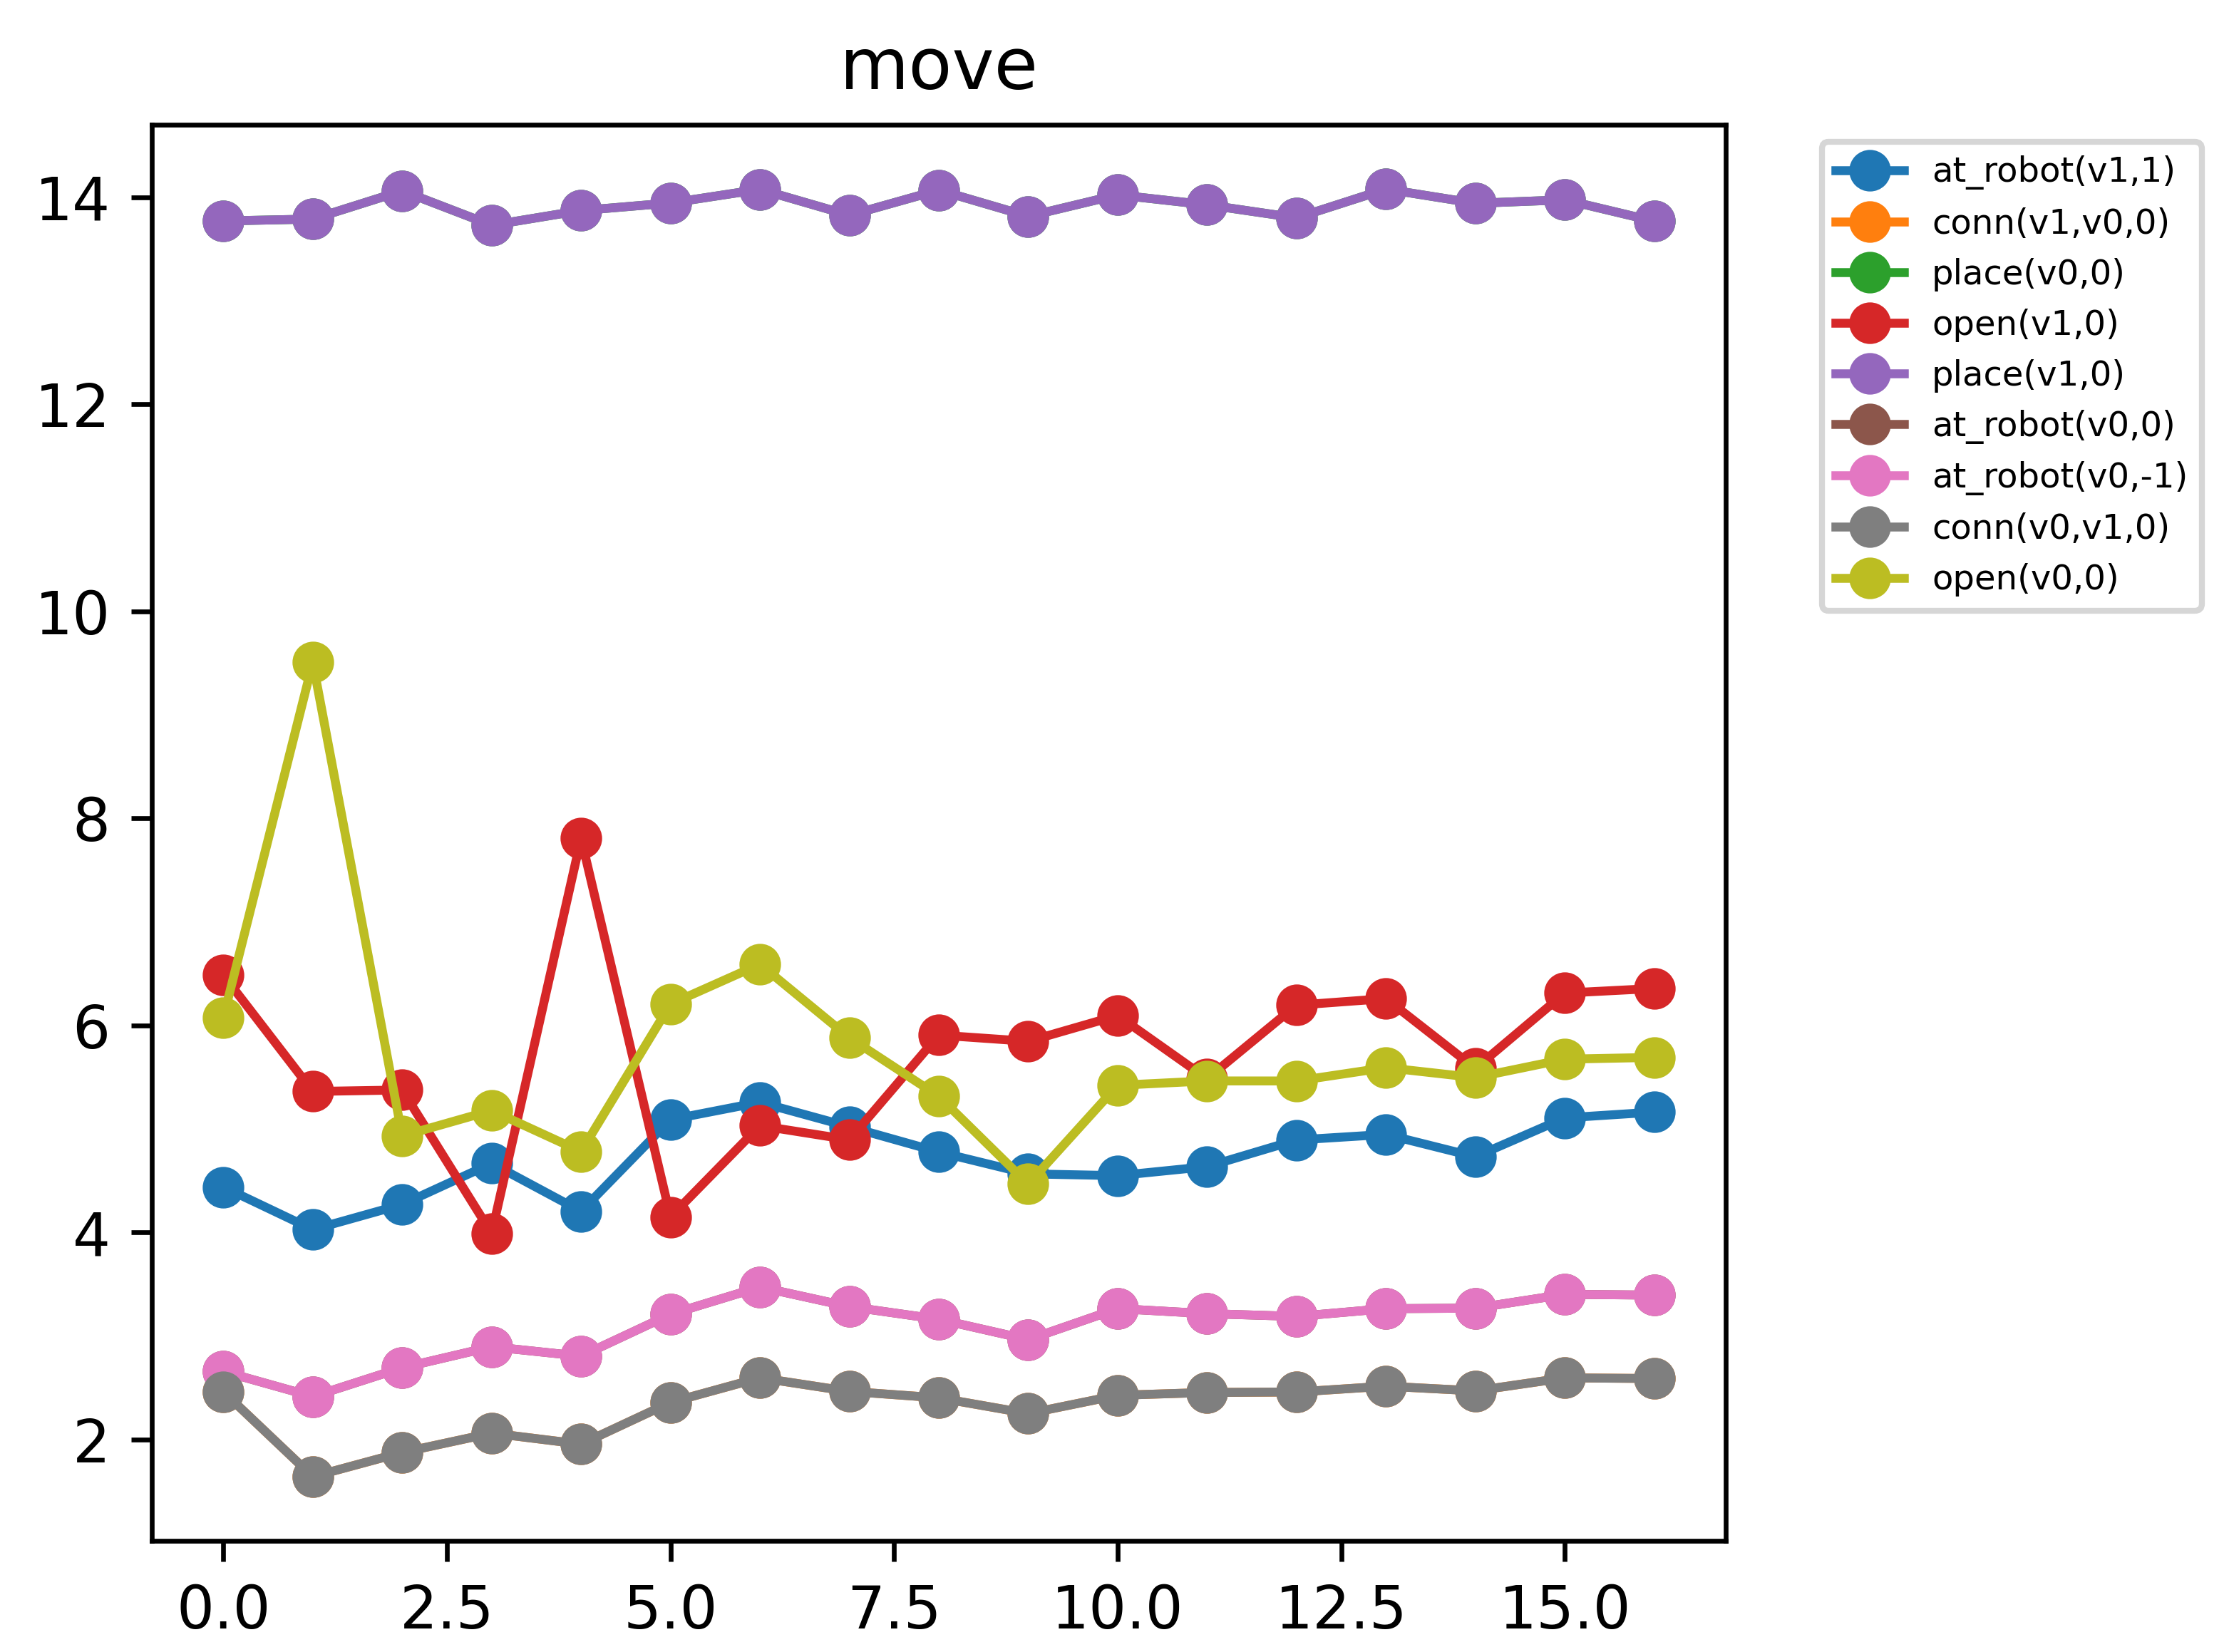
\includegraphics[width=1\textwidth]{images/tests/movegraph_100}
 \caption{Move action MLN, no noise {fig:mv 100}}

 \end{minipage}
 \hfill
 \begin{minipage}[b]{0.49\linewidth}

 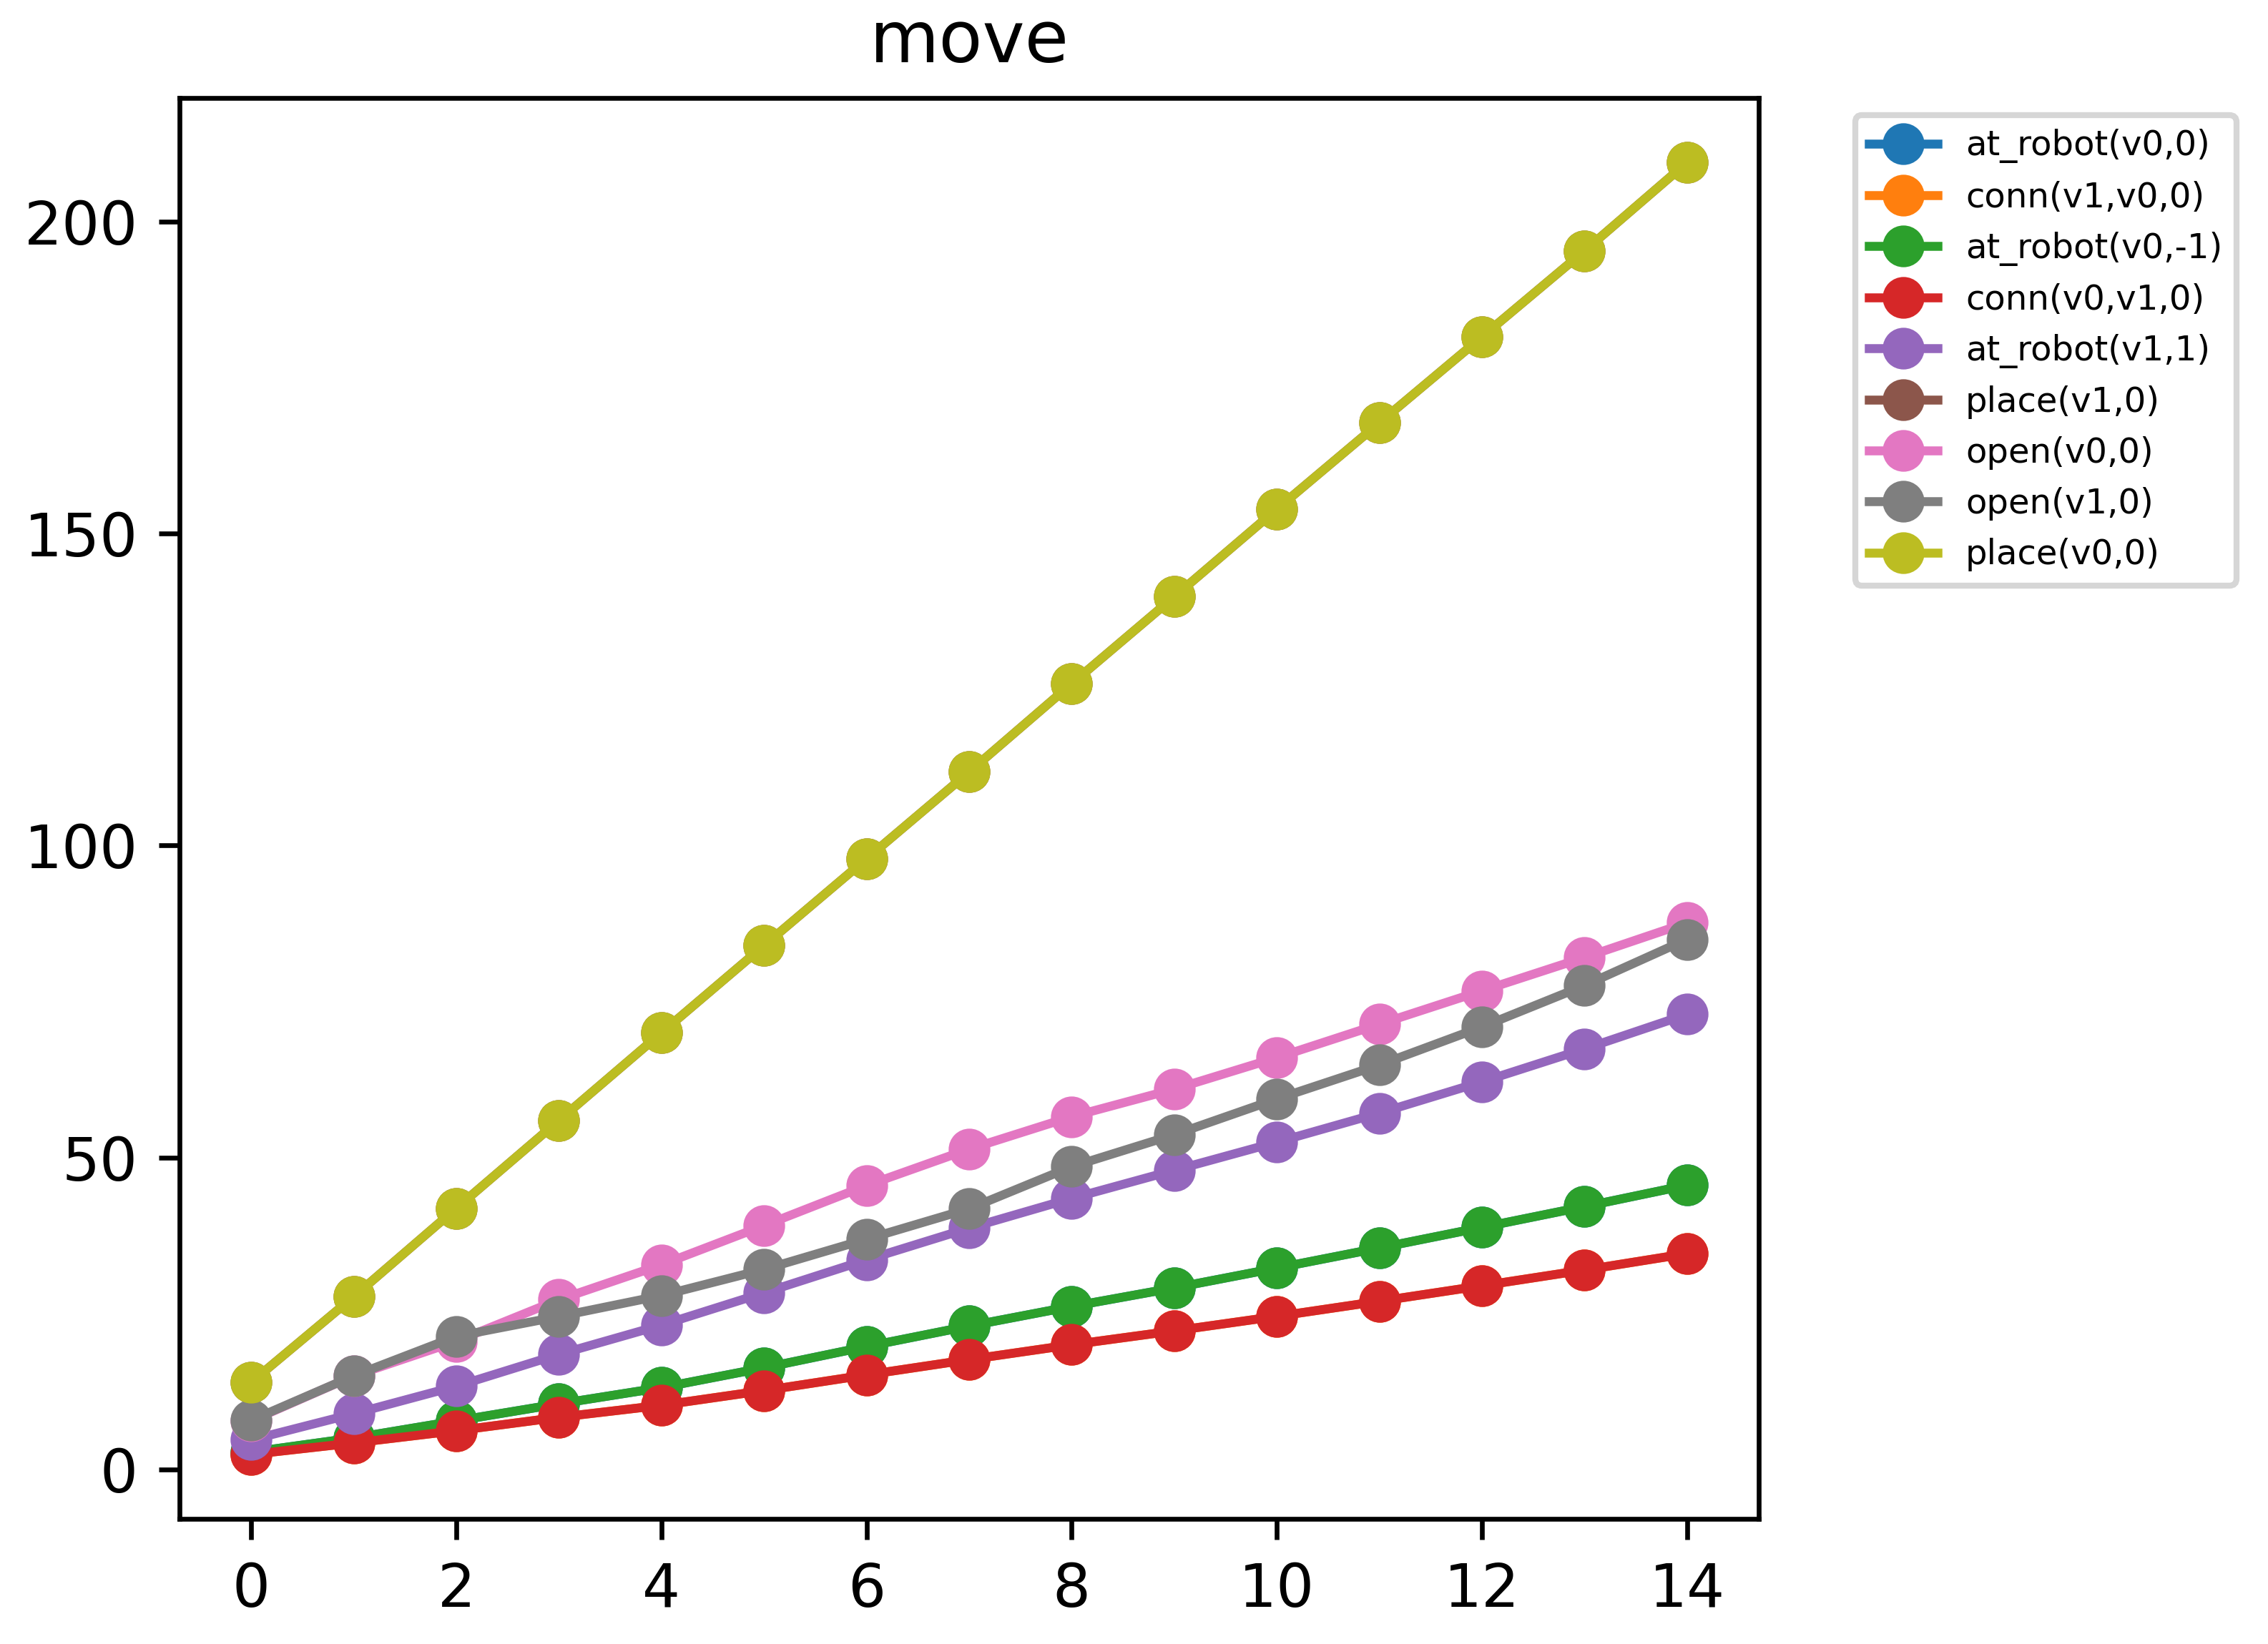
\includegraphics[width=1\textwidth]{images/tests/movegraph_100_cum}
 \caption{Move action MLN (cumulative), no noise {fig:mv 100 cum}}

 \end{minipage}
\end{figure}

\begin{figure}[h]
 \centering
 \begin{minipage}[b]{0.49\linewidth}
 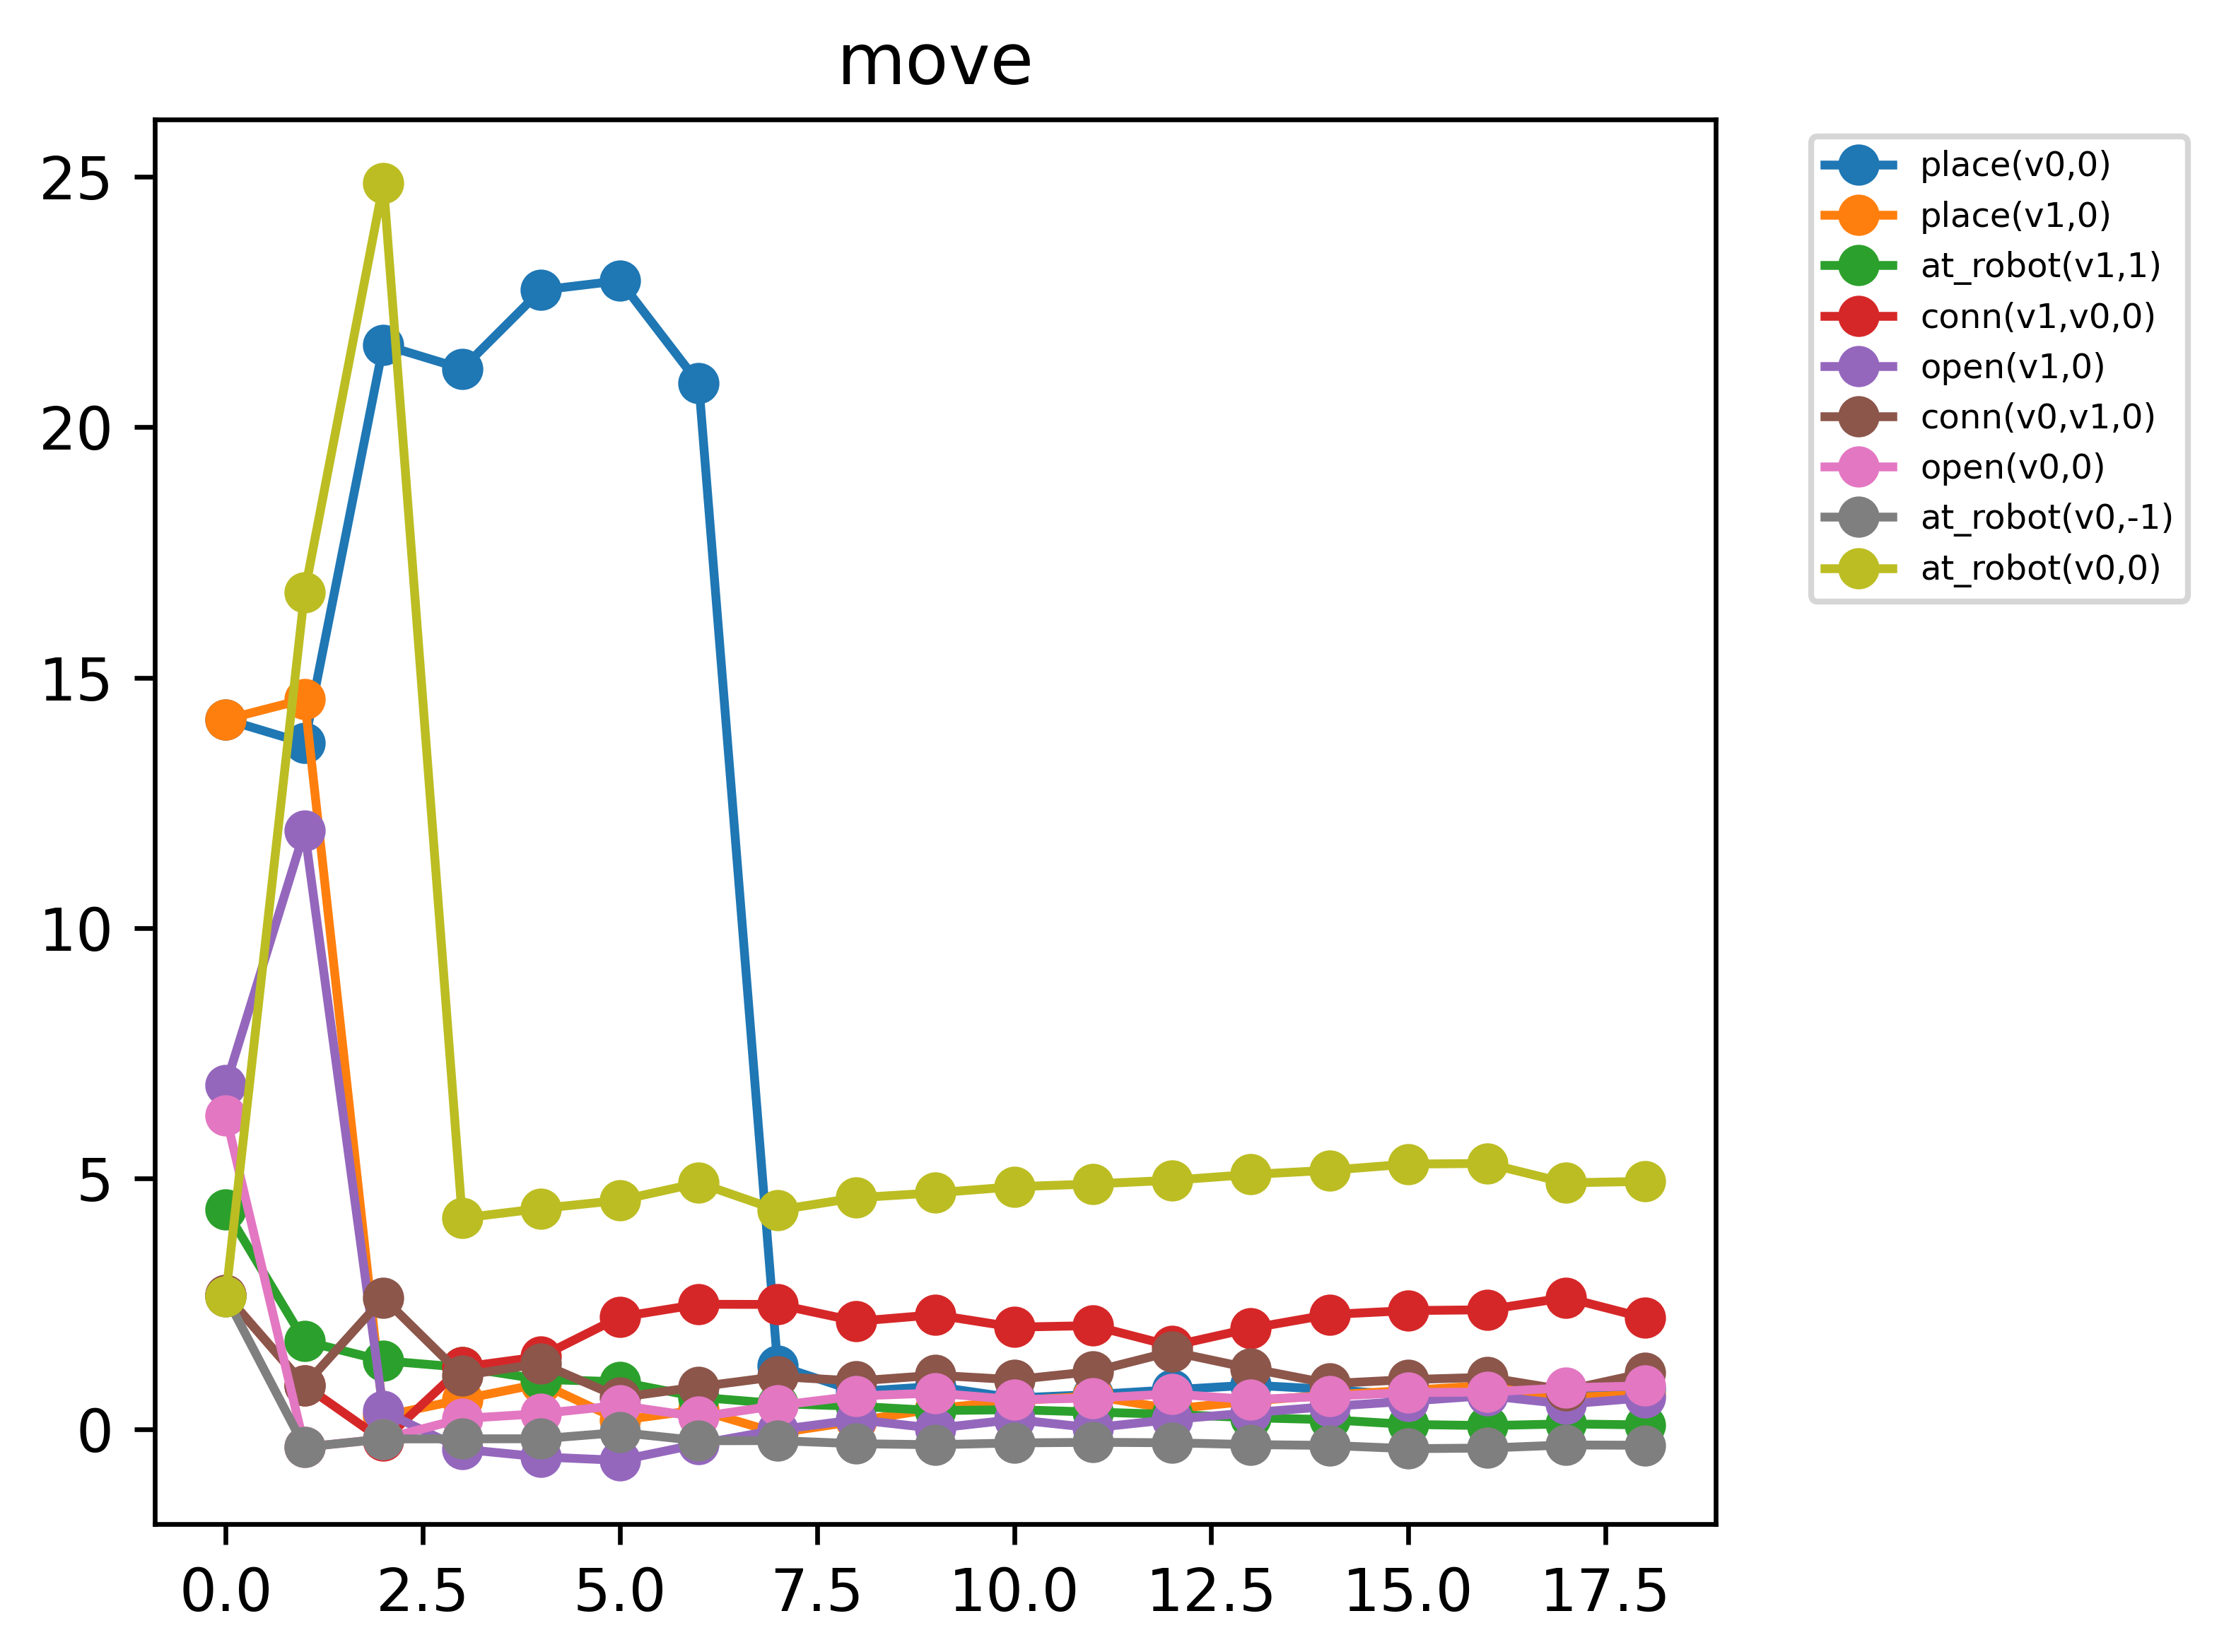
\includegraphics[width=1\textwidth]{images/tests/movegraph_rand_70}
 \caption{Move action MLN, .3 rand noise {fig:mv}}

 \end{minipage}
 \hfill
 \begin{minipage}[b]{0.49\linewidth}

 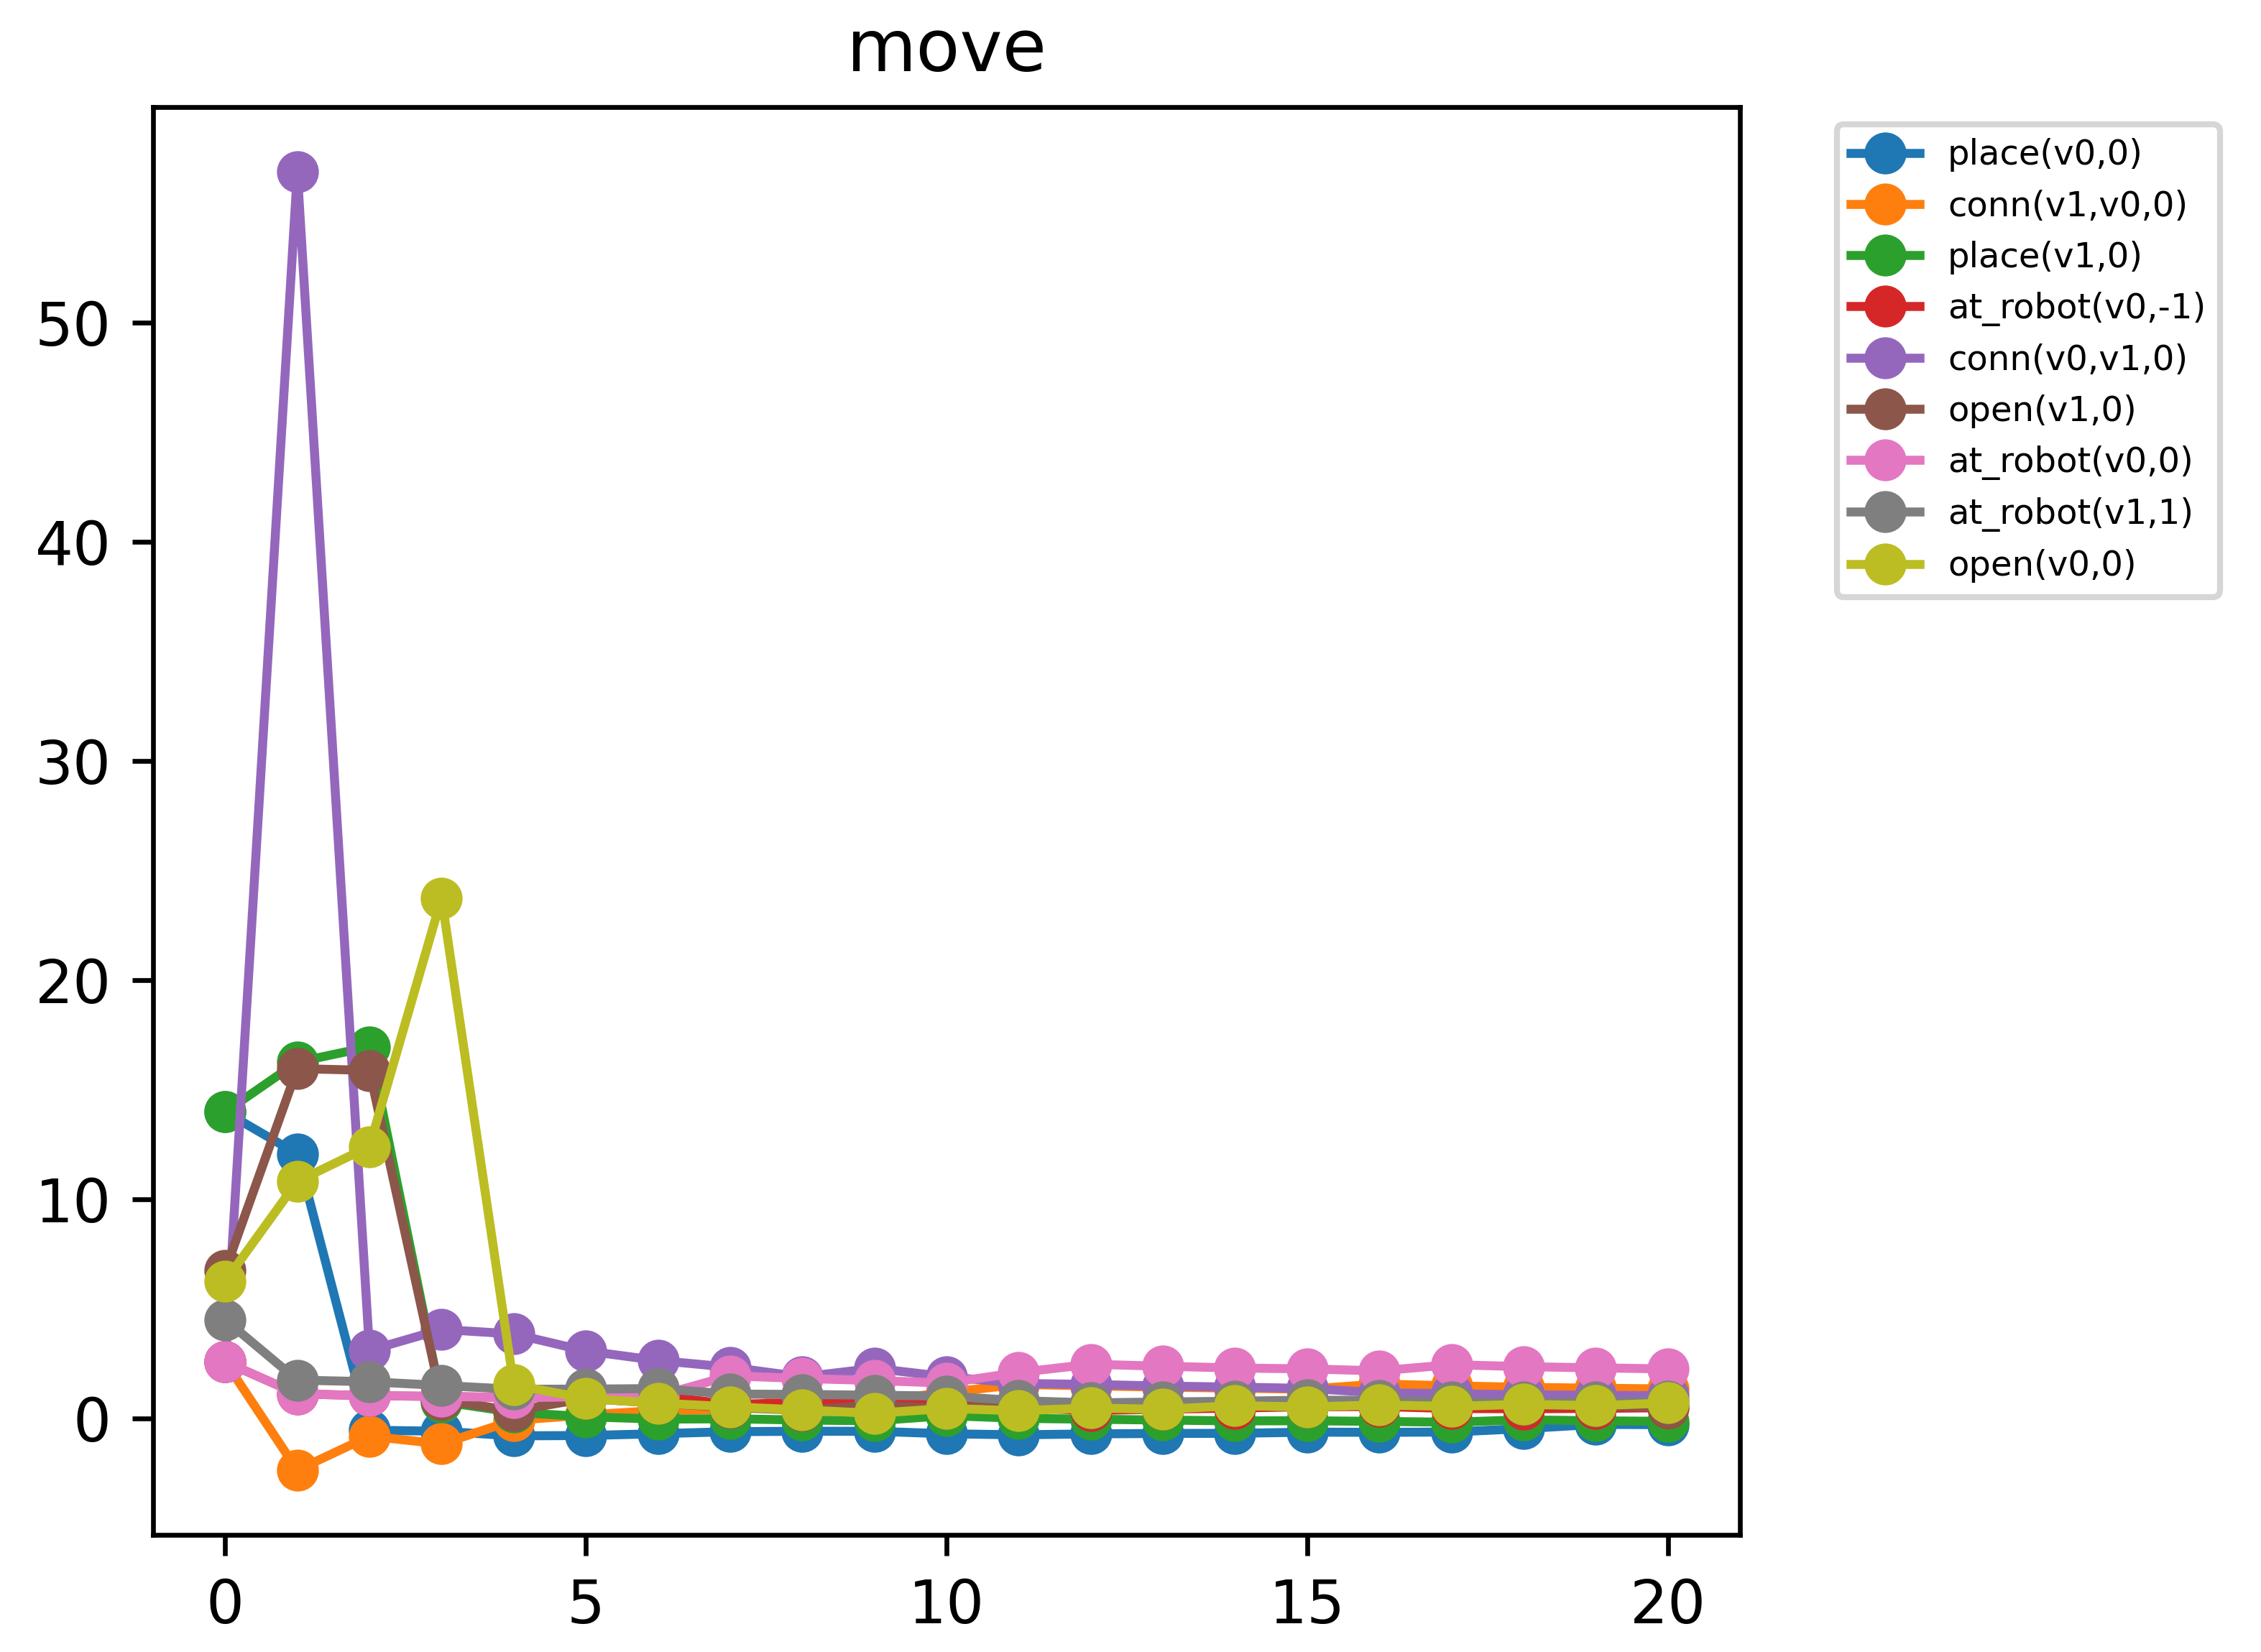
\includegraphics[width=1\textwidth]{images/tests/movegraph_rand_30}
 \caption{Move action MLN, .7 rand noise on){fig:mv_100_cum}}

 \end{minipage}
\end{figure}

\begin{figure}[h]
 \centering
 \begin{minipage}[b]{0.49\linewidth}
 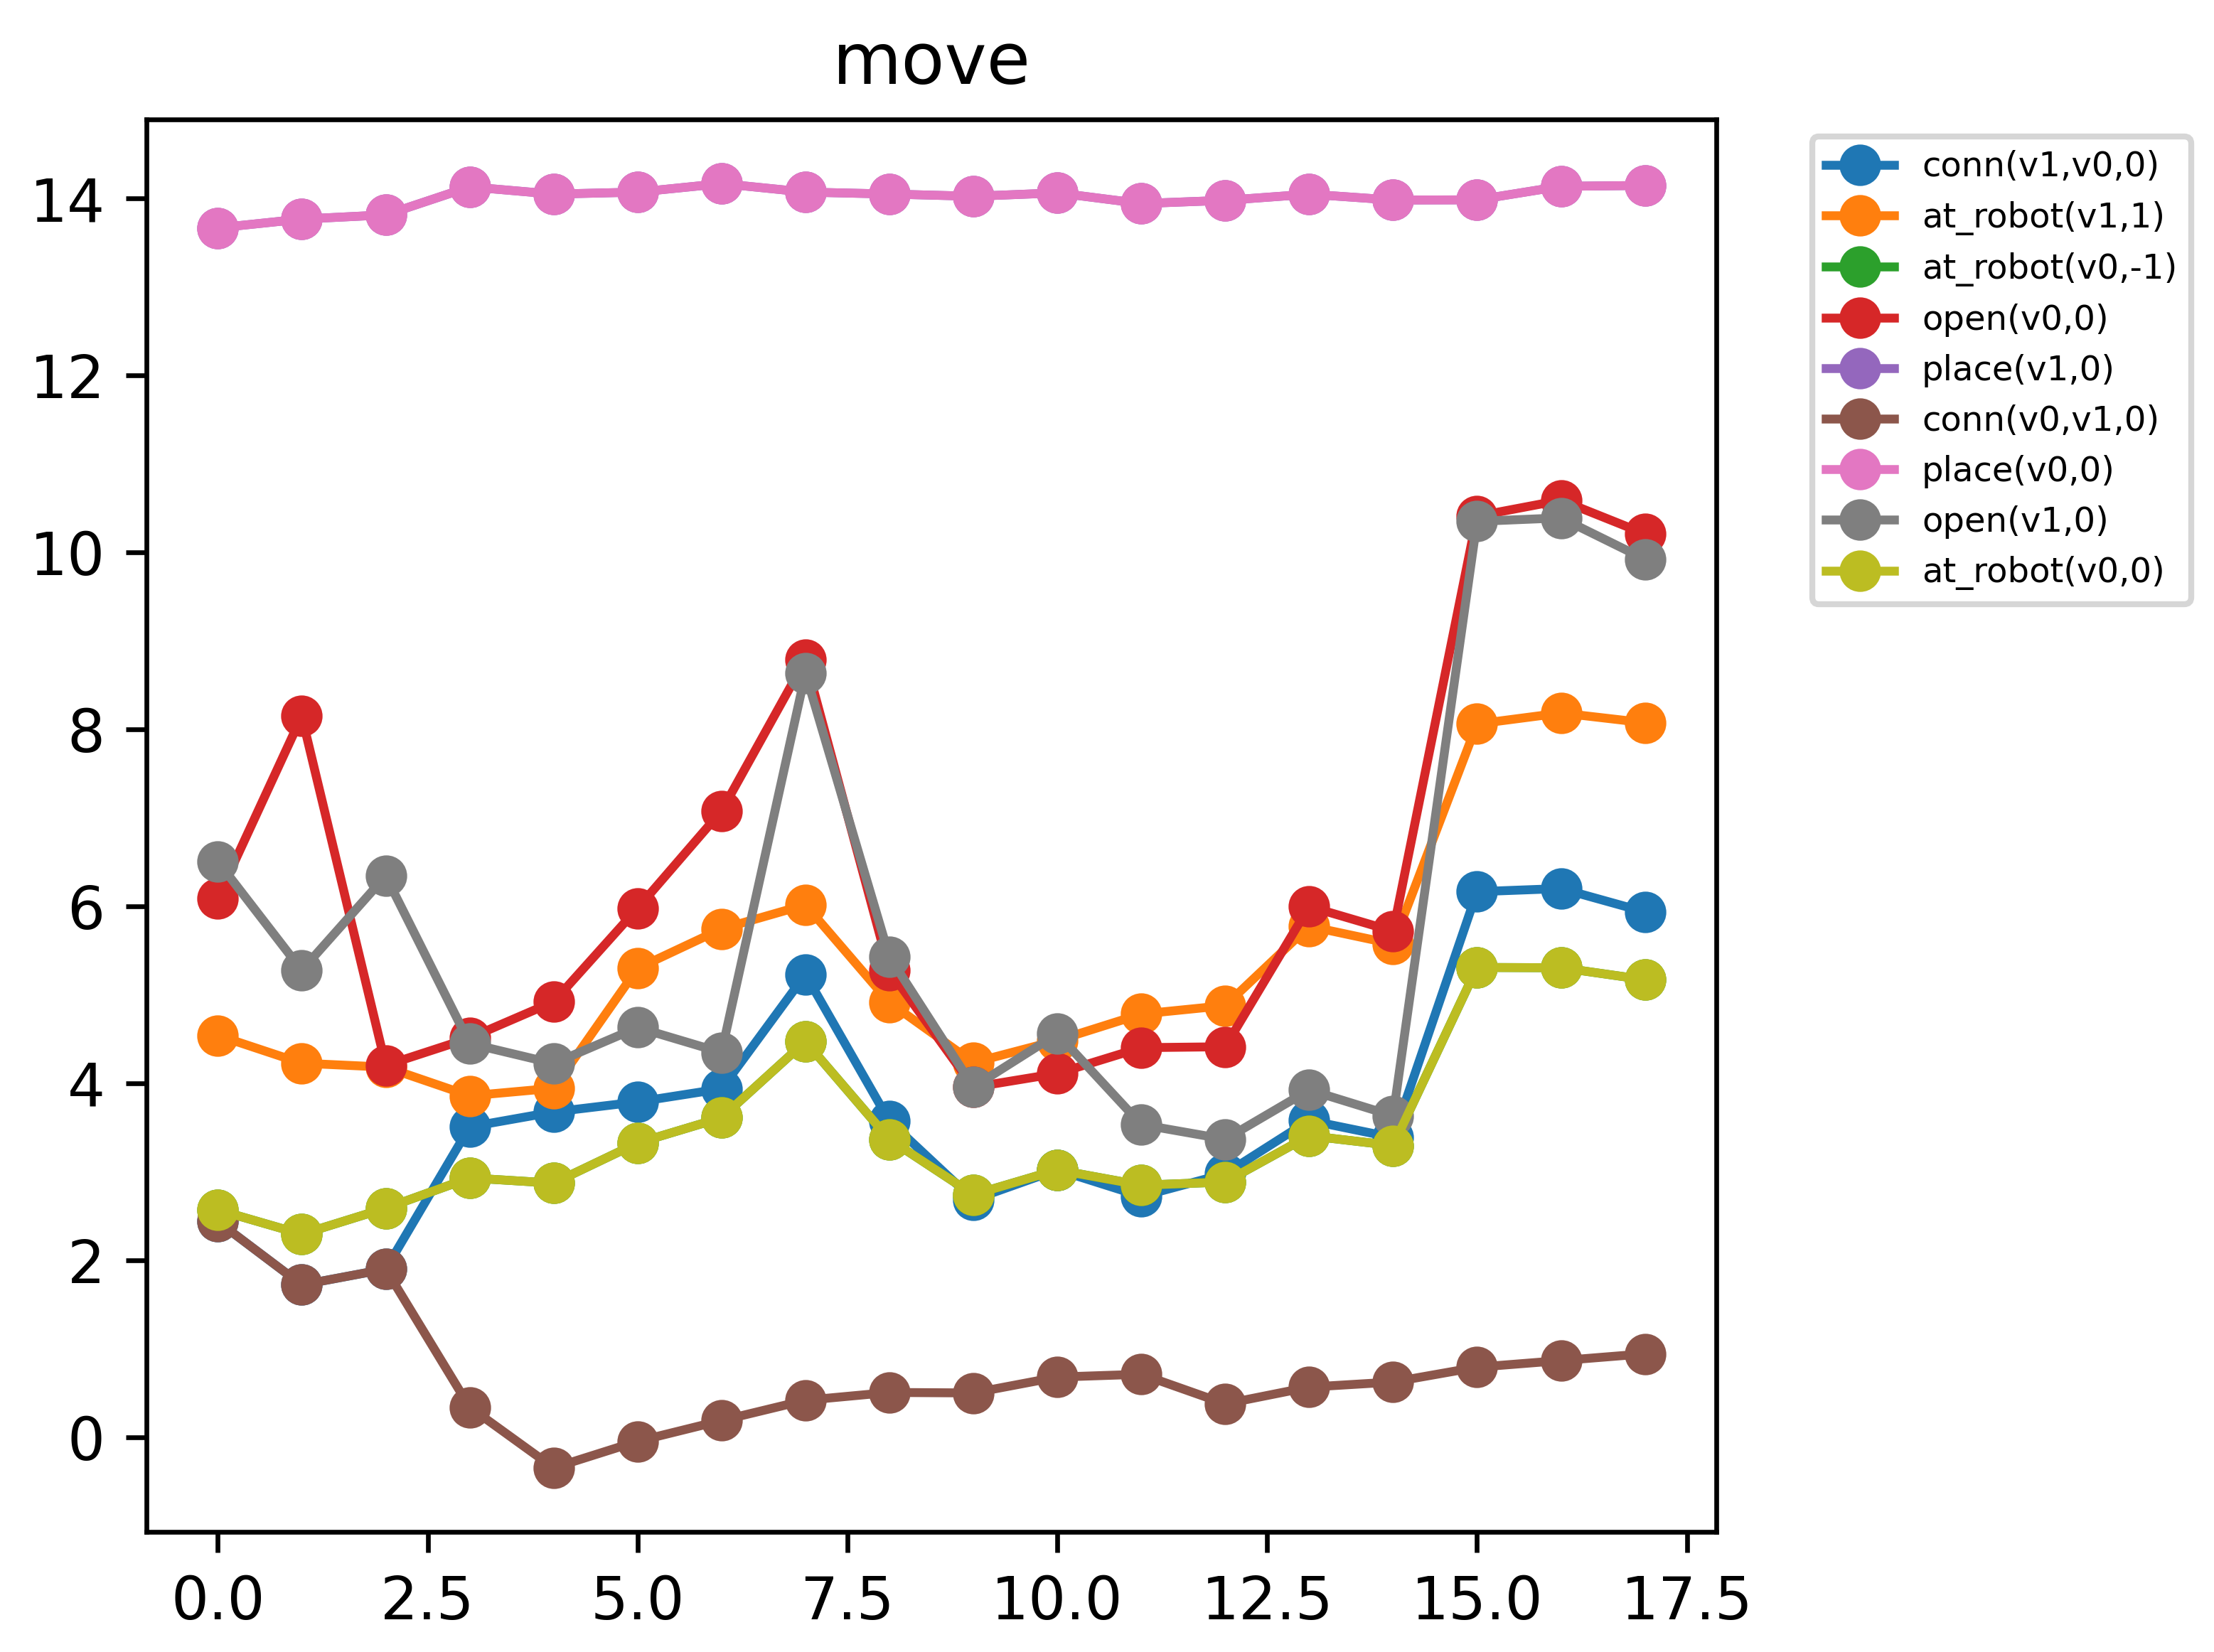
\includegraphics[width=1\textwidth]{images/tests/movegraph_sys_70}
 \caption{Move action MLN, .3 sys noise on conn(v0,v1,0) {fig:mv_100}}

 \end{minipage}
 \hfill
 \begin{minipage}[b]{0.49\linewidth}

 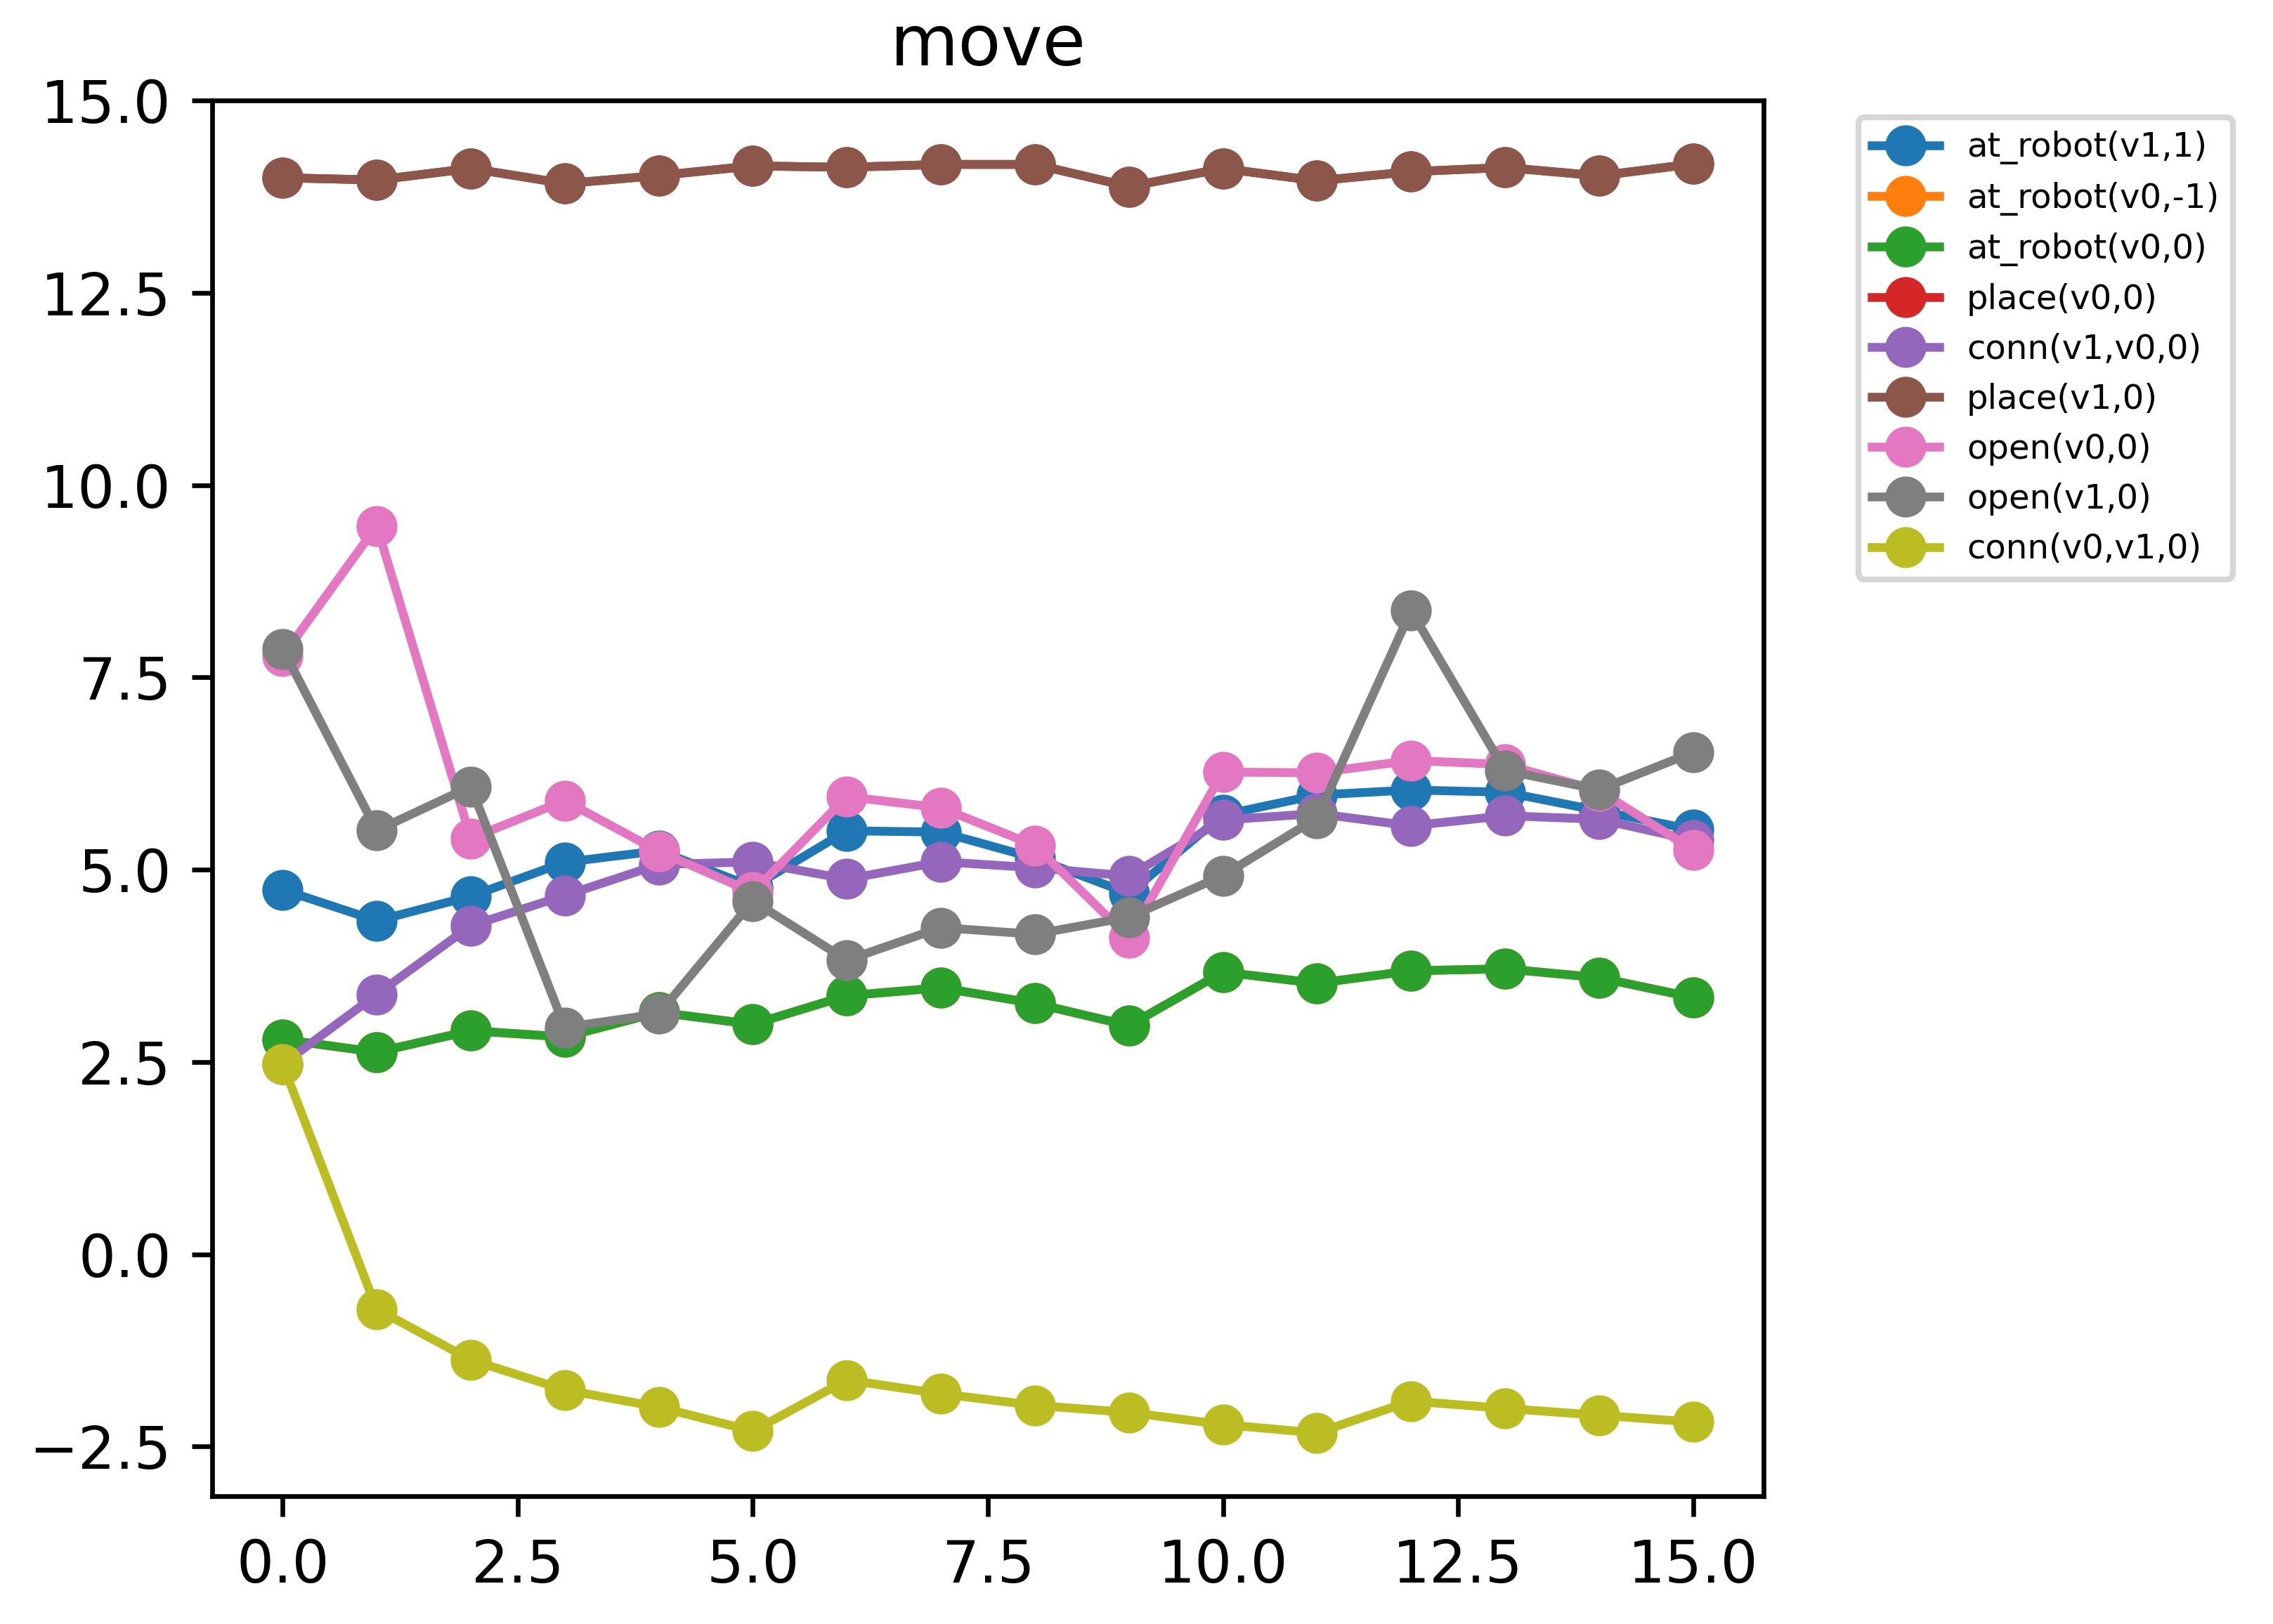
\includegraphics[width=1\textwidth]{images/tests/movegraph_sys_30}
 \caption{Move action MLN, .7 sys noise on conn(v0,v1,0){fig:mv_100_cum}}

 \end{minipage}
\end{figure}
\newpage
As we can observe from the above data, Although weights will reduce with noise. If we include predicates unrelated to the model, these will reduce much faster than noisy weights, this would allow us to recreate an action model from the network. \newline\newline
The greatest issue with this approach is not the viability of the technique but the efficiency of it. To train 25 database containing multiple actions, it takes around 30s to 1min, a multicore approach was not implemented in the pracmln package used for training, and a multitude of optimizations and fixes were done in order to speed up training and errors (optimizing data structures, operations over arrays, improperly handled exceptions, a fixed package has been uploaded to the project). A partial rewrite of the package for training MLN's online is required in order to use this technique on any moderately serious domains (>20 predicates). Optimizations include multithreading the training process, optimizing operation over grounded predicates and weights.\newline\newline
The results in the figures provided were created by training MLN's on pruned weights as forgoing this step made training impossible. Training speed reduces significantly when the number of weights are doubled or tripled which is a common occurrence in a normal domain.